\documentclass[xcolor=pdftex,dvipsnames,table,mathserif,aspectratio=169]{beamer}
\usetheme{default}
\usetheme{metropolis}
\usepackage{mathtools}
\setbeamersize{text margin left=.3in,text margin right=.3in} 

\DeclarePairedDelimiter\abs{\lvert}{\rvert}%
\DeclarePairedDelimiter\norm{\lVert}{\rVert}%

\usepackage[english]{babel}
\usepackage{pgf,pgfarrows,pgfnodes,pgfautomata,pgfheaps}
\usepackage{amsmath,amssymb,setspace,centernot}
\usepackage[latin1]{inputenc}
\usepackage{pgf,tikz}
\usepackage[T1]{fontenc}
\usepackage{relsize}
\usepackage{pdfpages}
\usepackage[absolute,overlay]{textpos} 


\newenvironment{reference}[2]{% 
  \begin{textblock*}{\textwidth}(#1,#2) 
      \footnotesize\it\bgroup\color{red!50!black}}{\egroup\end{textblock*}} 

\DeclareMathSizes{10}{10}{6}{6} 

\begin{document}
\title{Multinomial Discrete Choice: Nested Logit and GEV}
\author{Chris Conlon}
\institute{Grad IO}
\date{\today}

\frame{\titlepage}

\begin{frame}
\frametitle{Multinomial Logit: IIA}
The multinomial logit is frequently criticized for producing unrealistic substitution patterns
\begin{itemize}
\item Suppose we got rid of a product $k$ then $s_{ij}(\mathcal{J}\setminus k) = s_{ij}(\mathcal{J})\cdot \frac{1}{1- s_{ik}}$.
\item Substitution is just proportional to your pre-existing shares $s_j$
\item No concept of ``closeness'' of competition!
\end{itemize}
\end{frame}


\begin{frame}
\frametitle{Can we do better?}
Multinomial Probit?
\begin{itemize}
\item The probit has $\varepsilon_i \sim N(0,\Sigma)$.
\item If $\Sigma$ is unrestricted, then this can produce relatively flexible substitution patterns.
\item Flexible is relative: still have normal tails, only pairwise correlations, etc.
\item It might be that $\rho_{12}$ is large if $1,2$ are similar products.
\item Much more flexible than Logit
\end{itemize}
Downside
\begin{itemize}
\item $\Sigma$ has potentially $J^2$ parameters (that is a lot)!
\item Maybe $J * (J-1)/2$ under symmetry. (still a lot).
\item Each time we want to compute $s_j(\theta)$ we have to simulate an integral of dimension $J$.
\item I wouldn't do this for $J \geq 5$.
\end{itemize}
\end{frame}




\begin{frame}
\frametitle{Relaxing IIA}
Let's make $\varepsilon_{ij}$ more flexible than IID. Hopefully still have our integrals work out.
\begin{eqnarray*}
u_{ij} =   V_{ij}  + \varepsilon_{ij}
\end{eqnarray*}
\begin{itemize}
\item One approach is to allow for a block structure on $\varepsilon_{ij}$ (and consequently on the elasticities).
\item We assign products into groups $g$ and add a group specific error term
\begin{eqnarray*}
u_{ij} =V_{ij}  + \eta_{g} + \varepsilon_{ij}
\end{eqnarray*}
\item The trick putting a distribution on $\eta_{ig} + \varepsilon_{ij}$ so that the integrals still work out.
\item Do not try this at home: it turns out the required distribution is a special case of \alert{GEV} (more on this later) and the resulting model is known as the \alert{nested logit}.
\end{itemize}
\end{frame}

\begin{frame}{Nested Logit}
A traditional (and simple) relaxation of the IIA property is the Nested Logit. This model is often presented as two sequential decisions.
\begin{itemize}
\item First consumers choose a category (following an IIA logit).
\item Within a category consumers make a second decision (following the IIA logit).
\item This leads to a situation where while choices within the same nest follow the IIA property (do not depend on attributes of other alternatives) choices among different nests do not!
\end{itemize}
\end{frame}

\begin{frame}{Alternative Interpretation}
\begin{figure}[htbp]
\begin{center}
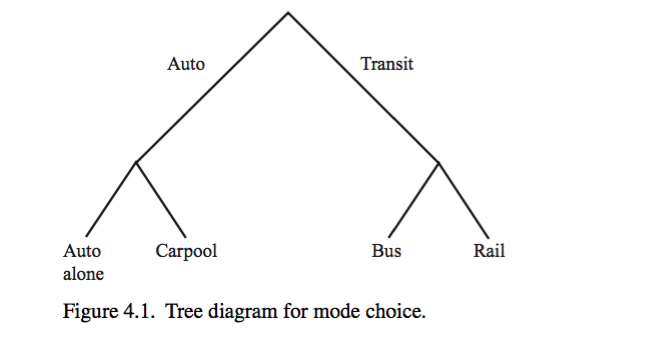
\includegraphics[width=5in]{resources/nesting.png}
\end{center}
\end{figure}
\end{frame}

\begin{frame}{Nested Logit}
Utility looks basically the same as before:
\begin{eqnarray*}
U_{ij} = V_{ij} + \underbrace{\eta_{ig} + \widetilde{\varepsilon_{ij}}}_{\varepsilon_{ij}(\lambda_g)}
\end{eqnarray*}
\begin{itemize}
\item We add a new term that depends on the group $g$ but not the product $j$ and think about it as varying unobservably over individuals $i$ just like $\varepsilon_{ij}$.
\item Now $\varepsilon_i \sim F(\varepsilon)$ where $F(\varepsilon) = \exp[-\sum_{g=G}^G \left(\sum_{j \in J_g} \exp[-\varepsilon_{ij}/\lambda_g]\right)^{\lambda_g}$. This is no longer Type I EV but a special kind of GEV.
\item The key is the addition of the $\lambda_g$ parameters which govern (roughly) the within group correlation.
\item This distribution is a bit cooked up to get a closed form result, but for $\lambda_g \in [0,1]$ for all $g$ it is consistent with random utility maximization.
\end{itemize}
\end{frame}

\begin{frame}{Nested Logit}
\small
The nested logit choice probabilities are:
\begin{eqnarray*}
s_{ij} = \frac{ e^{V_{ij}/\lambda_g} \left(\sum_{k \in J_g} e^{V_{ik}/\lambda_g} \right)^{\lambda_g -1}}{\sum_{h=1}^G \left(\sum_{k \in J_h} e^{V_{ik}/\lambda_h} \right)^{\lambda_h}}
\end{eqnarray*}
Within the same group $g$ we have IIA and proportional substitution 
\begin{eqnarray*}
\frac{s_{ij}}{s_{ik}} = \frac{ e^{V_{ij}/\lambda_g}}{ e^{V_{ik}/\lambda_g}}
\end{eqnarray*}

But for different groups we do not:
\begin{eqnarray*}
s_{ij} = \frac{ e^{V_{ij}/\lambda_g} \left(\sum_{k \in J_g} e^{V_{ik}/\lambda_g} \right)^{\lambda_g -1}}{ e^{V_{ik}/\lambda_h} \left(\sum_{k \in J_h} e^{V_{ik}/\lambda_h} \right)^{\lambda_h -1}}
\end{eqnarray*}
\end{frame}


\begin{frame}{Nested Logit}
We can take the probabilities and re-write them slightly with the substitution that 
$\log \left(\sum_{k \in J_g} e^{V_{ik}} \right)\equiv IV_{ig}=E_{\varepsilon}[\max_{j \in G} u_{ij}]$:
\begin{eqnarray*}
s_{ij} &=& \frac{ e^{V_{ij}/\lambda_g}}{ \left(\sum_{k \in J_g} e^{V_{ik}/\lambda_g} \right)}
\cdot
\frac{ \left(\sum_{k \in J_g} e^{V_{ik}/\lambda_g} \right)^{\lambda_g}}{\sum_{h=1}^G \left(\sum_{k \in J_h} e^{V_{ik}/\lambda_h} \right)^{\lambda_h}} \\
&=& \underbrace{\frac{ e^{V_{ij}/\lambda_g}}{ \left(\sum_{k \in J_g} e^{V_{ik}/\lambda_g} \right)}}_{s_{i j | g}}
\cdot
\underbrace{\frac{e^{\lambda_g IV_{ig}}}{\sum_{h=1}^{G} e^{\lambda_h IV_{ih}} }}_{s_{ig}}
\end{eqnarray*}
This is the decomposition into two logits that leads to the ``sequential logit'' story.
\end{frame}



\begin{frame}{Nested Logit : Notes}
\begin{itemize}
\item $\lambda_g=1$ is the simple logit case (IIA)
\item $\lambda_g \rightarrow 0$ implies that all consumers stay within the nest.
\item $\lambda < 0$ or $\lambda > 1$ can happen and usually means something is wrong. These models are not generally consistent with RUM. (If you report one in your paper I will reject it).
\item $\lambda$ is often interpreted as a correlation parameter and this is almost true but not exactly!
\item Because the nested logit can be written as the within group share $s_{ij|g}$ and the share of the group $s_{ig}$ we often explain this model as \alert{sequential choice}. It could just be a \alert{block structure} on $\varepsilon_i$.
\item You need to assign products to categories \alert{before you estimate} and you can't make mistakes!
\end{itemize}
\end{frame}

\begin{frame}
\frametitle{Parametric Identification}
Look at derivatives:
\begin{align*}
\frac{\partial\, s_{ij|g}}{\partial X_j} &= \beta_x \cdot s_{ij|g} \cdot (1-s_{ij|g}) \\
 \frac{\partial\, s_{ig}}{\partial X} &= (1-\lambda_g) \cdot \beta_x \cdot s_{ig}(1-s_{ig}) \\
  \frac{\partial\, s_{ig}}{\partial J} &= \frac{1-\lambda_g}{J} s_{ig}(1-s_{ig})
\end{align*}
\begin{itemize}
\item We get $\beta$ by changing $x_j$ within group
\item We get nesting parameter $\lambda$ by varying $X$
\item We don't have any parameters left to explain changing number of products $J$.
\item Estimation happens via MLE. This can be tricky because the model is non-convex. It helps to substitute $\tilde{\beta} = \beta/(1-\lambda_g)$
\end{itemize}
\end{frame}

\begin{frame}{A Confusing Gotcha}
An alternative version of the nested logit is popular in IO (Cardell 1991) $\sigma \approx \frac{1}{1-\lambda}$:
\begin{align*}
s_{ij | g}&=\frac{e^{V_{ij}/(1-\sigma)}}{D_{ig}}  \quad &
D_{ig}&= \log \left( \sum_{j \in \mathcal{G}} e^{V_{ij}/(1-\sigma)} \right)  \\
s_{ig}&=\frac{D_{ig}^{(1-\sigma)}}{\sum_{g} D_{ig}^{(1-\sigma)}} \quad &
s_{ij}=  s_{ij | g}\cdot s_{ig } &=\frac{\exp \left(\frac{V_{ij}}{1-\sigma}\right)}{D_{g}^{\sigma}\left[\sum_{g} D_{g}^{(1-\sigma)}\right]}
\end{align*}
Derivatives for nested logit are complicated and worked out at \url{http://www.nathanhmiller.org/nlnotes.pdf}.
\end{frame}

\begin{frame}
\frametitle{Substitution Patterns}
It is helpful to define: $Z(\sigma,s_g)=[\sigma + (1-\sigma) s_g ] \in (0,1]$ and note that $Z(0,s_g)=s_g$ and $Z(1,s_g)=1$. If two products are in the same nest or different nests respectively:
\begin{align*}
 -\frac{\frac{\partial s_{k}}{\partial p_j}}{\frac{\partial s_{j}}{\partial p_j} } \text{| same}
&=\frac{ s_{k|g} }{ Z^{-1}(\sigma,s_g) - s_{j|g}}  \equiv D_{jk}^{*}\\
 -\frac{\frac{\partial s_{k}}{\partial p_j}}{\frac{\partial s_{j}}{\partial p_j} } \text{| different}
&= \frac{ s_{k}  (1-\sigma) }{ 1 - s_{j|g} \cdot Z(\sigma,s_{g(j)}) } \equiv D_{jk}^{**}
\end{align*}
These are related by:
\begin{align*}
D_{jk}^{**}&=  D_{jk}^{*} \cdot \frac{s_{g(k)} \cdot (1-\sigma)}{Z(\sigma,s_{g(j)})}
\end{align*}
\end{frame}


\begin{frame}
\frametitle{GEV Variants}
There are more potential generalizations though they are less frequently used:
 \begin{itemize}
\item You can have multiple levels of nesting: first I select a size car (compact, mid-sized, full-sized) then I select a manufacturer, finally a car.
\item You can have potentially overlapping nests: Yogurt brands are one nest, Yogurt flavors are a second nest. This way strawberry competes with strawberry and/or Dannon substitutes for Dannon.
 \end{itemize}
\end{frame}

\begin{frame}{McFadden (1978) and GEV}
In case you are wondering where these things come from...
\begin{align*}
s_{ij}(\mathcal{J})=\frac{y_{j}\cdot  \frac{\partial G_i}{\partial y_{j}}\left(y_{i1}, \ldots, y_{iJ}\right)}{\mu \cdot G\left(y_{i1}, \ldots, y_{iJ}\right)}
\end{align*}
With conditions on the \alert{generator function} $G$:
\begin{enumerate}
\item $G(\cdot)$ is homogenous of degree $\mu > 0$ so that $G(\alpha y)=\alpha^{\mu} G(y)$
\item $\lim _{y_{j} \rightarrow+\infty} G\left(y_{1}, \ldots, y_{j}, \ldots, y_{J}\right)=+\infty, \text { for each } j \in \mathcal{J} $
\item the $k$ th partial derivative with respect to $k$ distinct $y_{j}$ is \alert{non-negative if $k$ is
odd} and \alert{non-positive if $k$ is even} that is, for any distinct indices $i_{1}, \ldots, i_{k} \in \mathcal{J}$, we have
$$
(-1)^{k} \frac{\partial^{k} G}{\partial x_{i_{1}} \ldots \partial x_{i_{k}}}(x) \leq 0, \forall x \in \mathbb{R}_{+}^{J}
$$
\end{enumerate}
The objects are more mathematical than economic...
\end{frame}



\begin{frame}{McFadden (1978) and GEV}
This is much easier with an example:
\begin{align*}
s_{ij}(\mathcal{J})=\frac{y_{j}\cdot  \frac{\partial G_i}{\partial y_{j}}\left(y_{i1}, \ldots, y_{iJ}\right)}{\mu \cdot G_i\left(y_{i1}, \ldots, y_{iJ}\right)}
\end{align*}
\begin{itemize}
\item If $y_j = e^{V_{ij}}$ and $G_i = \log \sum_{j \in \mathcal{J}} e^{V_{ij}}$ we get the IIA logit.
\item If $y_j = e^{V_{ij}}$ and $G_i=\sum_{h=1}^{H}\left(\sum_{j \in B_{h}} Y_{ij}^{1 / \lambda_{h}}\right)^{\lambda_{h}}$ we get the nested logit.
\item ... if $G_i=\sum_{h=1}^{H}\left(\sum_{j \in B_{h}}\left(\alpha_{j h} Y_{ij}\right)^{1 / \lambda_{k}}\right)^{\lambda_{k}}$ we get \alert{generalized nested logit} (GNL).
\item ... if $G=\sum_{k=1}^{J-1} \Sigma_{l=k+1}^{J}\left(y_{i k}^{1 / \lambda_{k l}}+y_{i l}^{1 / \lambda_{k l}}\right)^{\lambda_{k l}}$ we get \alert{pairwise combinatorial logit} (PCL).
\item there are a number of other \alert{cross nested logit} variants with slightly different setups (from each other).
\end{itemize}
\end{frame}



\begin{frame}{GEV and Variants}
What's next?
\begin{itemize}
\item Many of these GEV and variants are found in the engineering literature (particularly traffic problems, civil engineering, and industrial engineering).
\item Economists tend to use either nested logit or mixed logit (next lecture).
\item Part of the issue is that it is hard to understand the restrictions on the $G$ function and the economic meaning of the patterns produced by some of these models.
\item But they may be more parsimonious and easier to estimate than the alternatives.
\end{itemize}
\end{frame}


\end{document}